\documentclass[aspectratio=169]{beamer}
%%%%%%%%%%%%%%%%%%%%%%%%%%%%%%%%%%%%%%%%%
% Beamer Presentation
% LaTeX Template
% Version 1.0 (10/11/12)
%
% This template has been downloaded from:
% http://www.LaTeXTemplates.com
%
% License:
% CC BY-NC-SA 3.0 (http://creativecommons.org/licenses/by-nc-sa/3.0/)
%
%%%%%%%%%%%%%%%%%%%%%%%%%%%%%%%%%%%%%%%%%

%----------------------------------------------------------------------------------------
%	PACKAGES AND THEMES
%----------------------------------------------------------------------------------------

\usepackage[portuges]{babel}
\usepackage[utf8]{inputenc}
\usepackage[alf]{abntex2cite}	
\usepackage[portuguese, linesnumbered, vlined, titlenumbered, ruled]{algorithm2e}
\SetKwRepeat{Registro}{registro \{}{\}}%
\usepackage{beamerthemesplit}
\usepackage{multirow}
\usepackage{scalefnt}

% The Beamer class comes with a number of default slide themes
% which change the colors and layouts of slides. Below this is a list
% of all the themes, uncomment each in turn to see what they look like.

%\usetheme{default}
%\usetheme{AnnArbor}
%\usetheme{Antibes}
%\usetheme{Bergen}
%\usetheme{Berkeley}
%\usetheme{Berlin}
%\usetheme{Boadilla}
%\usetheme{CambridgeUS}
%\usetheme{Copenhagen}
%\usetheme{Darmstadt}
%\usetheme{Dresden}
%\usetheme{Frankfurt}
%\usetheme{Goettingen}
%\usetheme{Hannover}
%\usetheme{Ilmenau}
%\usetheme{JuanLesPins}
%\usetheme{Luebeck}
\usetheme{Madrid}
%\usetheme{Malmoe}
%\usetheme{Marburg}
%\usetheme{Montpellier}
%\usetheme{PaloAlto}
%\usetheme{Pittsburgh}
%\usetheme{Rochester}
%\usetheme{Singapore}
%\usetheme{Szeged}
%\usetheme{Warsaw}

% As well as themes, the Beamer class has a number of color themes
% for any slide theme. Uncomment each of these in turn to see how it
% changes the colors of your current slide theme.

%\usecolortheme{albatross}
%\usecolortheme{beaver}
%\usecolortheme{beetle}
%\usecolortheme{crane}
\usecolortheme{dolphin}
%\usecolortheme{dove}
%\usecolortheme{fly}
%\usecolortheme{lily}
%\usecolortheme{orchid}
%\usecolortheme{rose}
%\usecolortheme{seagull}
%\usecolortheme{seahorse}
%\usecolortheme{whale}
%\usecolortheme{wolverine}

%\setbeamertemplate{footline} % To remove the footer line in all slides uncomment this line
%\setbeamertemplate{footline}[page number] % To replace the footer line in all slides with a simple slide count uncomment this line

%\setbeamertemplate{navigation symbols}{} % To remove the navigation symbols from the bottom of all slides uncomment this line


\usepackage{graphicx} % Allows including images
\usepackage{booktabs} % Allows the use of \toprule, \midrule and \bottomrule in tables

%----------------------------------------------------------------------------------------
%	TITLE PAGE
%----------------------------------------------------------------------------------------

\title[Árvores Binárias]{Algoritmos e Estrutura de Dados}
\subtitle{Árvores Binárias}
\author[Frederico Santos de Oliveira]{prof. Frederico Santos de Oliveira}
\institute[UFMT]{Universidade Federal de Mato Grosso\\ Faculdade de Engenharia}
\date{}

\begin{document}

%------------------------------------------------
\begin{frame}
\titlepage % Print the title page as the first slide

\begin{figure}[!h]
  \centering
   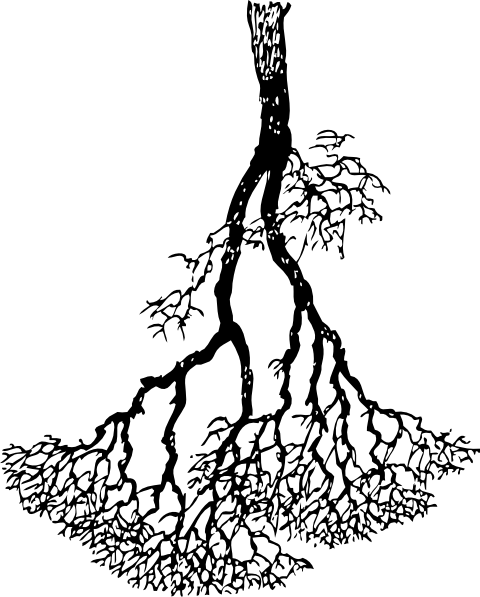
\includegraphics[width=80pt]{imagens/introducao.png}
  \label{fig_introducao}
\end{figure}
\end{frame}

%------------------------------------------------

\begin{frame}
\frametitle{Roteiro} % Table of contents slide, comment this block out to remove it
\tableofcontents % Throughout your presentation, if you choose to use \section{} and \subsection{} commands, these will automatically be printed on this slide as an overview of your presentation
\end{frame}

%----------------------------------------------------------------------------------------
%	PRESENTATION SLIDES
%----------------------------------------------------------------------------------------

%------------------------------------------------
\section{Objetivos}

\begin{frame}
\frametitle{Objetivos}

Esta aula tem como objetivos:

\begin{enumerate}
\item Apresentar os conceitos básicos sobre árvores;
\item Exemplificar os algoritmos de manipulação de árvores por meio de pseudo-códigos.
\end{enumerate}

\end{frame}

%------------------------------------------------
% 
% \section{Referências bibliográficas}
%   \frame{\frametitle{Referências bibliográficas}
%     \bibliographystyle{abntex2-alf}
%     \bibliography{referencias}
%   }
%   
%------------------------------------------------
\section{Introdução} % Sections can be created in order to organize your presentation into discrete blocks, all sections and subsections are automatically printed in the table of contents as an overview of the talk
%------------------------------------------------

\begin{frame}
\frametitle{Introdução}
\begin{itemize}
 \item Uma árvore é uma abstração matemática usada para representar estruturas hierárquicas não lineares dos objetos modelados.
 \item É definida usando um conjunto de nodos (ou vértices) e arestas, que são utilizadas para conectar qualquer par de nodos ou vértices.
 \item Basicamente, qualquer problema em que exista algum tipo de hierarquia pode ser representado por uma árvore.
\end{itemize}
\end{frame}

%------------------------------------------------
\begin{frame}{Introdução}{Exemplo}
\begin{figure}[!h]
  \centering
   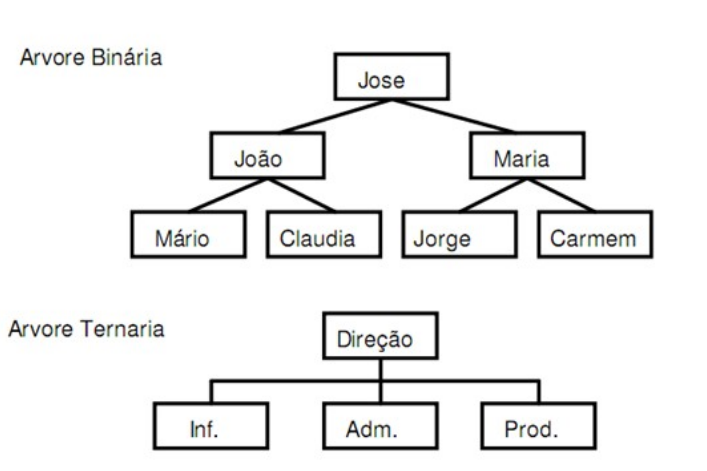
\includegraphics[width=200pt]{imagens/exemplo.png}
  \label{fig_exemplo}
\end{figure}
\end{frame}


%------------------------------------------------
\begin{frame}{Introdução}{Formas de Visualização}
\begin{figure}[!h]
  \centering
   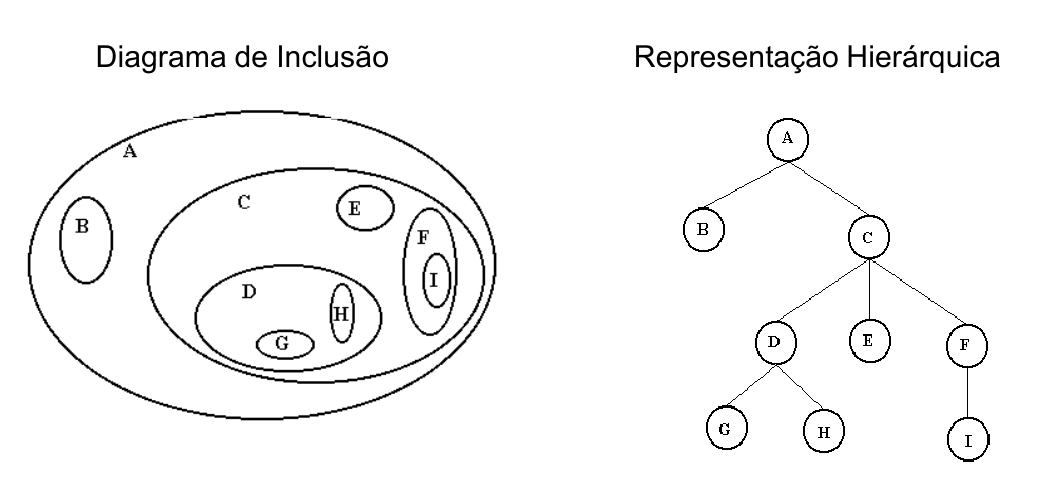
\includegraphics[width=250pt]{imagens/visualizacao.png}
  \label{fig_visualizacao}
\end{figure}
\end{frame}

% %------------------------------------------------
% \begin{frame}{Introdução}{Formas de Visualização}
% Representação por expressão parentetizada (Parênteses aninhados)
% \begin{itemize}
%  \item Cada conjunto de parênteses correspondentes contém um nodo e seus filhos.
%  \item Se um nodo não tem filhos, ele é seguido por um par de parênteses sem conteúdo.
%  \item Exemplo:
% \end{itemize}
% \centering{( A ( B ) ( C ( D ( G ) ( H )) ( E ) ( F ( I ))))}
% \end{frame}

\begin{frame}{Introdução}{Principais Conceitos}
\begin{block}{Grafo}
 Uma árvore é um tipo especial de grafo: um grafo {\bf não-direcionado}, {\bf conexo} e {\bf acíclico}. 
\end{block}
\begin{itemize}
 \item Uma árvore é formada por um conjunto de nodos ligados por arestas de forma hierárquica, simulando as árvores encontradas na natureza.
 \item Porém, nessa estrutura as árvores crescem de cima para baixo, ou seja, a raiz se encontra no topo e as folhas na parte mais baixa. 
\end{itemize}
\end{frame}

\begin{frame}{Introdução}{Principais Conceitos}
A seguir, a nomenclatura usada para se trabalhar com uma árvore:
\begin{itemize}
 \item {\bf Raiz}: é o nodo localizado na parte mais alta da árvore, o único que não possui pai.
 \item {\bf Pai}: também chamado de ancestral, é o nodo antecessor imediato de outro nodo.
 \item {\bf Filho}: é o nodo sucessor imediato de outro nodo.
\end{itemize}
\end{frame}

\begin{frame}{Introdução}{Principais Conceitos}
\begin{itemize}
 \item {\bf Nodo folha}: também chamado de nodo terminal, é qualquer nodo que não possui filhos.
 \item {\bf Nodo de derivação}: também chamado de nodo não-terminal, ou nodo interno, é qualquer nodo que possui ao menos um filho.
\end{itemize}
 \begin{figure}[!h]
  \centering
   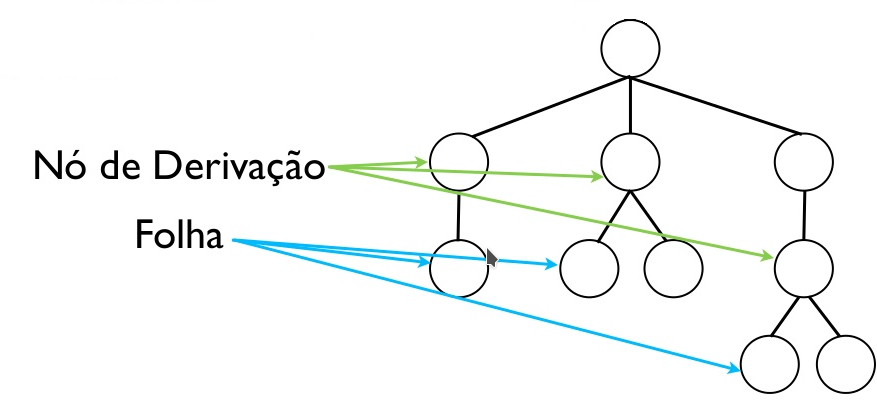
\includegraphics[width=200pt]{imagens/nodo_derivacao_interno.png}
  \label{fig_nodo_derivacao_interno}
\end{figure}
\end{frame}


\begin{frame}{Introdução}{Principais Conceitos}
\begin{itemize}
 \item {\bf Subárvores}:
 \begin{itemize}
 \item Dado um nodo da árvore, cada filho seu é considerado a raiz de uma nova subárvores.
 \item Qualquer nodo é a raiz de uma subárvore.
 \end{itemize}
 \begin{figure}[!h]
  \centering
   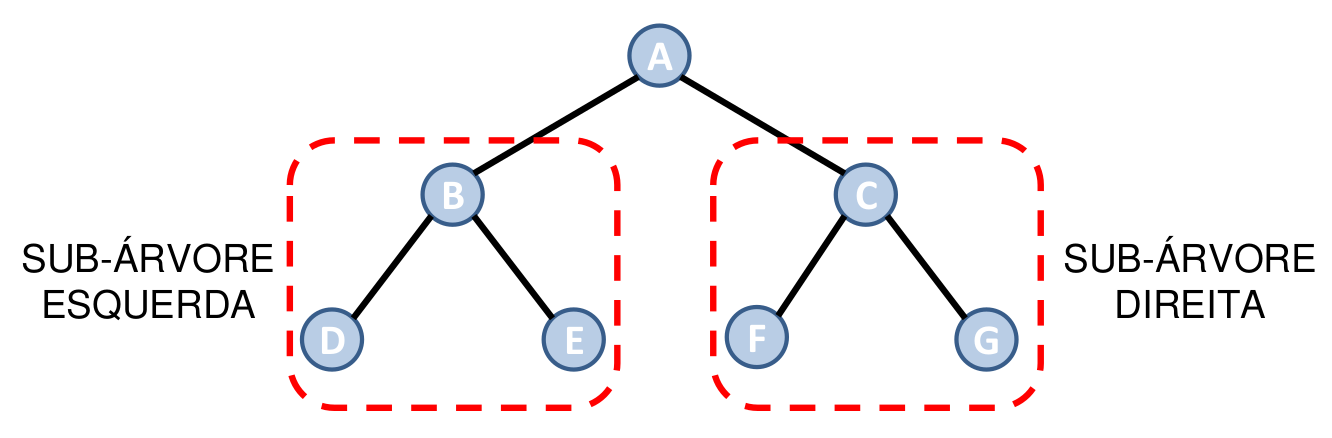
\includegraphics[width=250pt]{imagens/subarvores1.png}
  \label{fig_subarvores1}
\end{figure}
\end{itemize}
\end{frame}

\begin{frame}{Introdução}{Principais Conceitos}
 \begin{figure}[!h]
  \centering
   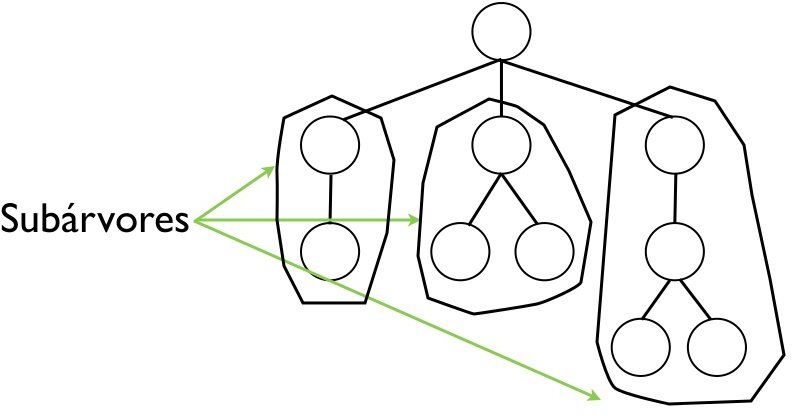
\includegraphics[width=250pt]{imagens/subarvores2.png}
  \label{fig_subarvores2}
\end{figure}
\end{frame}

\begin{frame}{Introdução}{Principais Conceitos}
\begin{itemize}
 \item {\bf Grau de um nodo}:
 \begin{itemize}
  \item O grau de um nodo é dado pelo número de subárvores que ele possui.
 \end{itemize}
 \item {\bf Grau de uma árvore}:
 \begin{itemize}
  \item É o maior valor dentre os graus de todos os seus nodos.
 \end{itemize} 
 \begin{figure}[!h]
  \centering
   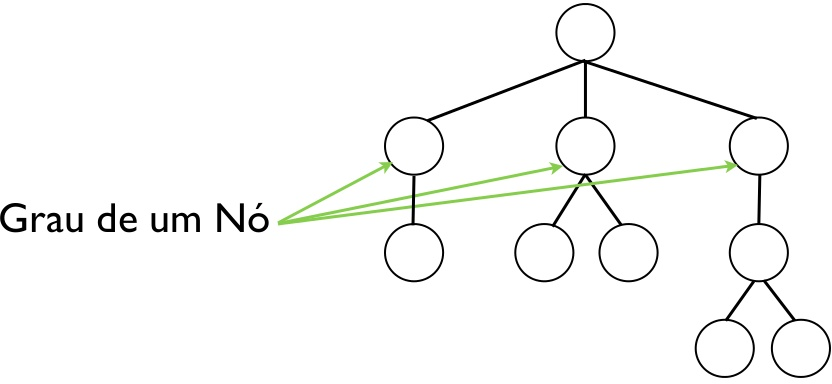
\includegraphics[width=200pt]{imagens/grau_arvore.png}
  \label{fig_grau_arvore}
\end{figure} 
\end{itemize}
\end{frame}

\begin{frame}{Introdução}{Principais Conceitos}
\begin{itemize}
 \item {\bf Caminho}: é uma sequência de nodos de modo que existe sempre uma aresta ligando o nodo anterior com o seguinte.
 \item {\bf Nível}: em uma árvore os nodos são classificados em diferentes níveis, começando a partir do nodo raiz (nível 0).
 \item {\bf Comprimento de um caminho}: quantidade de arestas em um caminho. 
\end{itemize}
 \begin{figure}[!h]
  \centering
   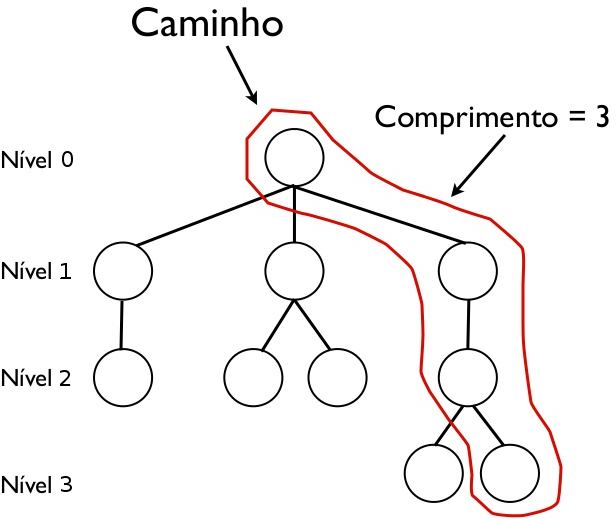
\includegraphics[width=150pt]{imagens/caminho.png}
  \label{fig_caminho}
\end{figure}
\end{frame}

\begin{frame}{Introdução}{Principais Conceitos}
\begin{itemize}
 \item {\bf Altura}:
 \begin{itemize}
 \item A altura (ou profundidade) de uma árvore é igual ao nível máximo de seus nodos.
 \item Ou seja, é o comprimento do caminho mais longo da raiz até uma das suas folhas.
 \item A altura de um nodo é igual ao comprimento do caminho do nodo até a raiz.
 \end{itemize}
\end{itemize}
\end{frame}

%------------------------------------------------
\begin{frame}{Introdução}{Principais Conceitos}
\begin{figure}[!h]
  \centering
   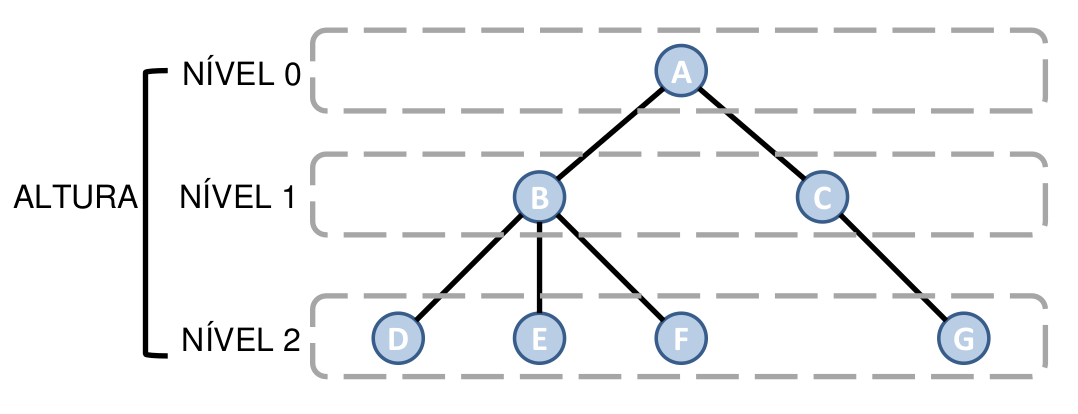
\includegraphics[width=250pt]{imagens/altura.png}
  \label{fig_altura}
\end{figure}
\end{frame}


%------------------------------------------------
\begin{frame}{Introdução}{Principais Conceitos}
\begin{figure}[!h]
  \centering
   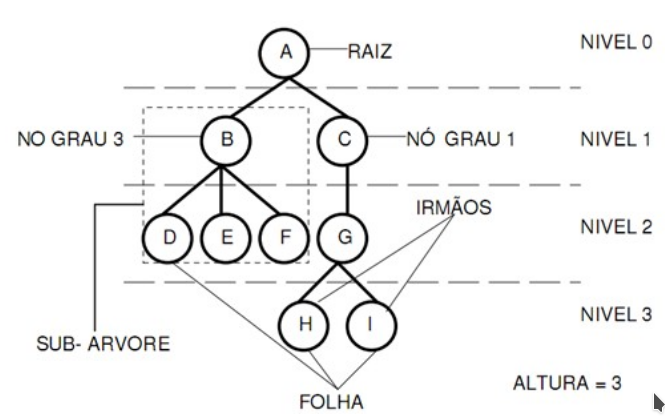
\includegraphics[width=200pt]{imagens/definicoes.png}
  \label{fig_definicoes}
\end{figure}
\end{frame}


\begin{frame}{Árvore Binária}{Exercício}
Considere a arvore a seguir:
\begin{figure}[!h]
  \centering
  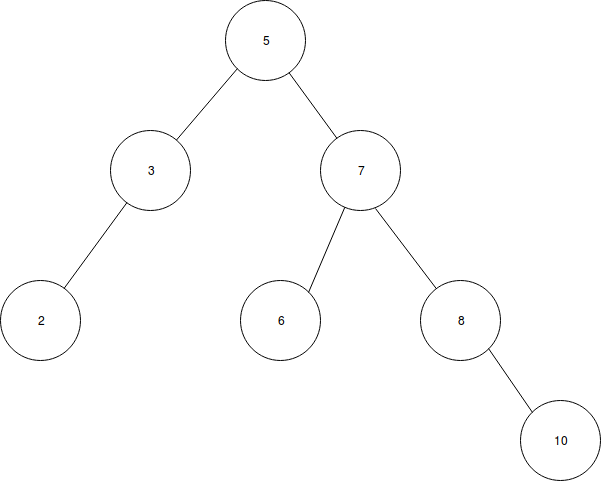
\includegraphics[width=140pt]{imagens/exercicio.png}
  \label{fig_exercicio_conceitos}
\end{figure}
\begin{itemize}
 \item Qual a altura do nodo com valor 6?
 \item Qual o grau do nodo com valor 3?
 \item Qual a altura da árvore?
 \item Qual o nível do nodo com valor 3?
 \item Qual o comprimento do caminho que liga o nodo 5 ao 8?
\end{itemize}
\end{frame}


\begin{frame}{Árvore Binária}{Exercício}
Considere a arvore a seguir:
\begin{figure}[!h]
  \centering
  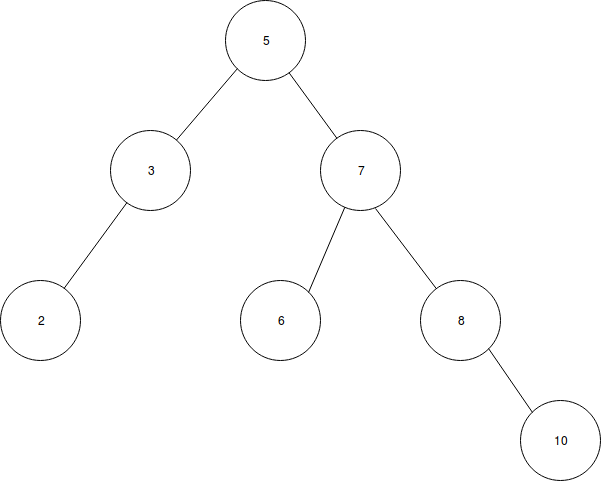
\includegraphics[width=140pt]{imagens/exercicio.png}
\end{figure}
\begin{itemize}
 \item Qual a altura do nodo com valor 6? {\bf Altura = 2}
 \item Qual o grau do nodo com valor 3? {\bf Grau = 1}
 \item Qual a altura da árvore? {\bf Altura = 3}
 \item Qual o nível do nodo com valor 3? {\bf Nível = 1}
 \item Qual o comprimento do caminho que liga o nodo 5 ao 8? {\bf Comp. = 2}
\end{itemize}
\end{frame}

\section{Árvore Binária}

\begin{frame}{Árvore Binária}
\begin{itemize}
 \item Uma árvore binária é um tipo especial de árvore em que cada nodo pode possuir no máximo duas subárvores: a subárvore da {\bf esquerda} e a da {\bf direita}.
 \item Caso o nodo possua nenhuma subárvore, este será um nodo folha.
 \item Exemplo:
\end{itemize}
\begin{figure}[!h]
  \centering
   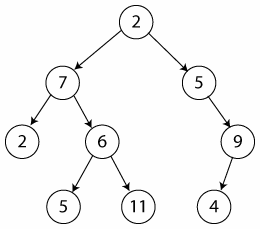
\includegraphics[width=100pt]{imagens/exemplo_arvore_binaria.png}
  \label{fig_exemplo_arvore_binaria}
\end{figure}
\end{frame}

\begin{frame}{Árvore Binária}{Classificação}
Tipos de Árvore Binária
\begin{itemize}
 \item {\bf Estritamente Binária}: é uma árvore binária em que cada nodo tem 0 ou 2 filhos.
 \item {\bf Completa}: é aquela em se $n$ é um nodo com algumas de subárvores vazias, então $n$ se localiza no penúltimo ou no último nível. 
  \item {\bf Cheia}: é uma árvore em que se um nodo tem alguma subárvore vazia então ele está no último nível.
\end{itemize}
\end{frame}

% --------------------------------------------------------------------

\begin{frame}{Árvore Binária}{Classificação}
Exemplos:
\begin{figure}[!h]
  \centering
  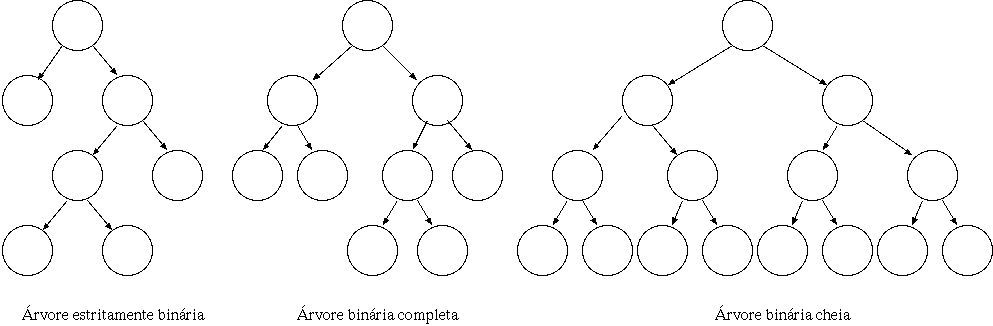
\includegraphics[width=350pt]{imagens/classificacao.png}
  \label{fig_classificacao}
\end{figure}
\end{frame}

% --------------------------------------------------------------------

\begin{frame}{Árvore Binária}{Classificação}
Árvore Binária Cheia
 \begin{figure}[!h]
  \centering
   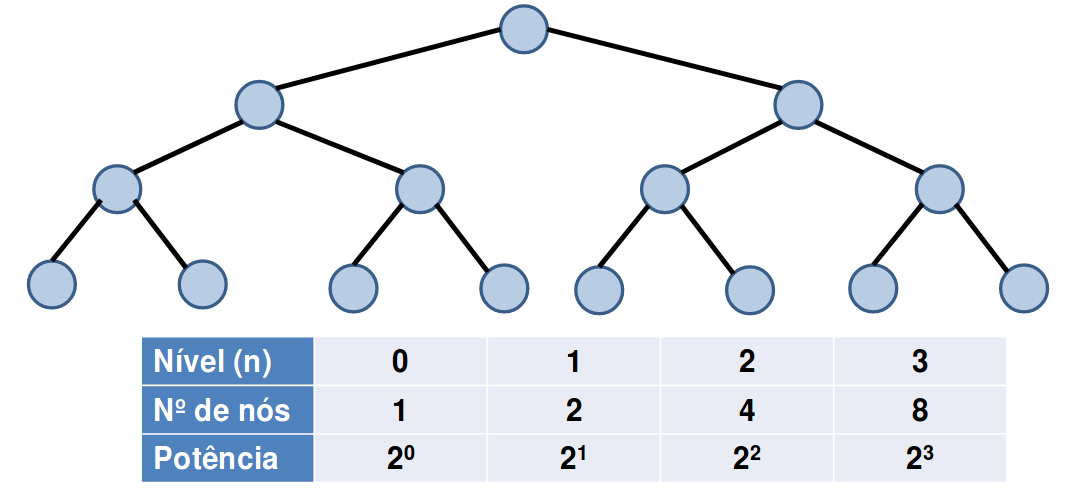
\includegraphics[width=250pt]{imagens/arvore_binaria_cheia.png}
  \label{fig_arvore_binaria_cheia}
\end{figure}
\end{frame}

% --------------------------------------------------------------------

\begin{frame}{Árvore Binária}{Classificação}
Na árvore cheia é possível calcular o número de nodos por nível, assim como o número total de nodos:
\begin{itemize}
 \item Um nível $i$ possui exatamente $2^i$ nodos.
 \item Se um nível $i$ possui $n$ nodos, o nível $i+1$ possui $2n$ nodos.
 \item Uma árvore de altura $h$ possui $2^{h+1} - 1$ nodos.
\end{itemize}
\end{frame}

% --------------------------------------------------------------------
\section{Implementação}
% --------------------------------------------------------------------

\subsection{Estrutura Nodo}

\begin{frame}{Árvore Binária}{Implementação}
A estrutura {\bf nodo} contém três campos:
\begin{itemize}
 \item Um ponteiro {\bf esq}, que indica o filho da esquerda daquele nodo.
 \item Um ponteiro {\bf dir}, que indica o filho da direita daquele nodo.
 \item Um campo {\bf item} do tipo {\bf int}, que é o tipo de dado a ser armazenado no nodo da árvore.
\end{itemize}
\begin{figure}[!h]
  \centering
  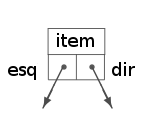
\includegraphics[width=70pt]{imagens/nodo.png}
  \label{fig_nodo}
\end{figure}
\end{frame}


\begin{frame}[fragile]{Árvore Binária}{Estrutura Nodo}
\begin{algorithm}[H]
\caption{Nodo} 
\label{Nodo}
\Inicio{
 \Registro{Nodo}{
    Inteiro: item; \\
    Ponteiro Nodo: esq; \\
    Ponteiro Nodo: dir; 
  }
}
\end{algorithm} 
\end{frame}

\subsection{Estrutura Árvore Binária}

\begin{frame}{Árvore Binária}{Implementação}
A estrutura {\bf árvore} trata-se de um ponteiro do tipo {\bf nodo}:
\begin{itemize}
 \item O ponteiro {\bf raiz} aponta para o nodo raiz da árvore.
 \item Se a árvore está vazia, o ponteiro {\bf raiz} aponta para NULL.
\end{itemize}
\begin{figure}[!h]
  \centering
  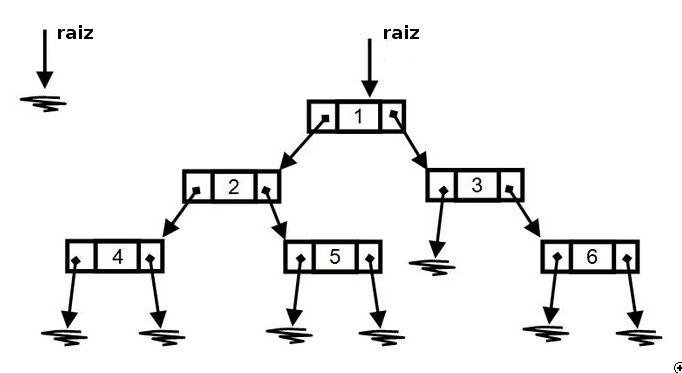
\includegraphics[width=300pt]{imagens/estrutura_arvore.png}
  \label{fig_estrutura_arvore}
\end{figure}
\end{frame}


%------------------------------------------------

\subsection{Algoritmo CriaÁrvore | ÁrvoreVazia}

\begin{frame}{Árvore Binária}{Implementação}
% \scalebox{0.5}{
\begin{algorithm}[H]
\caption{CriaÁrvore} 
\label{CriaArvore}
\Entrada{Ponteiro $r$ para raiz.}
\Inicio{
  r $\leftarrow$ NULL \\
}
\end{algorithm}
% }  
\begin{algorithm}[H]
\caption{ÁrvoreVazia} 
\label{ArvoreVazia}
\Entrada{Ponteiro $r$ para raiz.}
\Saida{V ou F}
\Inicio{
  \Se {(r = NULL)} {
    \Retorna V
  }
  \Senao {
    \Retorna F
  }
  
}
\end{algorithm}
% }  
\tiny{Adaptado de \cite{Backes2016}}
\end{frame}

%------------------------------------------------
\subsection{Algoritmo QuantidadeNodos}

\begin{frame}{Árvore Binária}{Implementação}
A quantidade de nodos em uma árvore com raiz em $r$ é calculada da seguinte forma:
 \begin{itemize}
 \item Verifica se $r$ é vazio. 
 \begin{itemize}
 \item Caso sim, a quantidade de nodos é zero.
 \item Caso contrário, o total de nodos da árvore com raiz em $r$ será a soma da quantidade de nodos em suas subárvores mais um (referente ao nodo raiz $r$).
 \end{itemize} 
 \item A seguir, o pseudocódigo.
 \end{itemize} 
\end{frame}

\begin{frame}{Árvore Binária}{Implementação}
% \scalebox{0.5}{
\begin{algorithm}[H]
\caption{QuantidadeNodos} 
\label{QuantidadeNodos}
\Entrada{Ponteiro $r$ para raiz.}
\Saida{Quantidade de nodos em $r$.}
\Inicio{
  \Se {(r = NULL)} {
    \Retorna 0
  }
  \Senao {
    total\_esq $\leftarrow$ QuantidadeNodos($r$.esq) \\
    total\_dir $\leftarrow$ QuantidadeNodos($r$.dir) \\
    \Retorna total\_esq + total\_dir + 1
  }
}
\end{algorithm}
% }  
\tiny{Adaptado de \cite{Backes2016}}
\end{frame}

%------------------------------------------------

\subsection{Algoritmo AlturaÁrvore}

\begin{frame}{Árvore Binária}{Implementação}
A altura é calculada da seguinte forma:
 \begin{itemize}
 \item Verifica se o nodo é um nodo folha. 
 \begin{itemize}
 \item Caso sim, sua altura é zero. Nesse caso, a altura de seus filhos é -1.
 \item Caso contrário, obtém-se a maior altura entre suas subárvores, e incrementa em um.
 \end{itemize} 
 \item A seguir, o pseudocódigo.
 \end{itemize} 
\end{frame}

\begin{frame}{Árvore Binária}{Implementação}
% \scalebox{0.5}{
\begin{algorithm}[H]
\caption{AlturaÁrvore} 
\label{AlturaArvore}
\Entrada{Ponteiro $r$ para raiz.}
\Saida{Altura da árvore com raiz em $r$.}
\Inicio{
  \Se {(r = NULL)} {
    \Retorna { -1 }
  }
  \Senao {
    alt\_esq $\leftarrow$ AlturaÁrvore($r$.esq) \\
    alt\_dir $\leftarrow$ AlturaÁrvore($r$.dir) \\
    \Se {(alt\_esq $>$ alt\_dir)} {
      \Retorna alt\_esq + 1
    }
    \Senao {
      \Retorna alt\_dir + 1
    }
  }
}
\end{algorithm}
% }  
\tiny{Adaptado de \cite{Backes2016}}
\end{frame}

% -----------------------------------

\subsection{Percurso em Árvore}

\begin{frame}{Árvore Binária}{Percurso em Árvore}
\begin{itemize}
 \item Não existe uma ordem ``natural'' para se percorrer todos os de uma árvore binária.
 \item Apesar disso, existem algumas formas muito utilizadas para se percorrer uma árvore. 
 \item São elas:
 \begin{itemize}
 \item Percurso {\bf pré-ordem}: visita a raiz, o filho da esquerda e o filho da direita.
 \item Percurso {\bf em-ordem}: visita o filho da esquerda, a raiz e o filho da direita.
 \item Percurso {\bf pós-ordem}: visita o filho da esquerda, o filho da direita e a raiz.
 \end{itemize} 
\end{itemize}
\end{frame}

%------------------------------------------------

\begin{frame}{Árvore Binária}{Implementação}
% \scalebox{0.5}{
\begin{algorithm}[H]
\caption{PercursoPréOrdem} 
\label{PercursoPreOrdem}
\Entrada{Ponteiro $r$ para raiz.}
\Inicio{
  \Se {(r $\neq$ NULL)} {
    Imprima (r.item) \\
    PercursoPréOrdem(r.esq)\\
    PercursoPréOrdem(r.dir)\\
  }
}
\end{algorithm}
% }  
\tiny{Adaptado de \cite{Backes2016}}
\end{frame}

%------------------------------------------------

\begin{frame}{Árvore Binária}{Implementação}
% \scalebox{0.5}{
\begin{algorithm}[H]
\caption{PercursoEmOrdem} 
\label{PercursoEmOrdem}
\Entrada{Ponteiro $r$ para raiz.}
\Inicio{
  \Se {(r $\neq$ NULL)} {
    PercursoEmOrdem(r.esq)\\
    Imprima (r.item) \\    
    PercursoEmOrdem(r.dir)\\
  }
}
\end{algorithm}
% }  
\tiny{Adaptado de \cite{Backes2016}}
\end{frame}

%------------------------------------------------

\begin{frame}{Árvore Binária}{Implementação}
% \scalebox{0.5}{
\begin{algorithm}[H]
\caption{PercursoPósOrdem} 
\label{PercursoPosOrdem}
\Entrada{Ponteiro $r$ para raiz.}
\Inicio{
  \Se {(r $\neq$ NULL)} {
    PercursoPósOrdem(r.esq)\\ 
    PercursoPósOrdem(r.dir)\\
    Imprima (r.item) \\       
  }
}
\end{algorithm}
% }  
\tiny{Adaptado de \cite{Backes2016}}
\end{frame}

% -----------------------------------

\begin{frame}{Árvore Binária}{Percurso em Árvore}

\begin{figure}[!h]
  \centering
  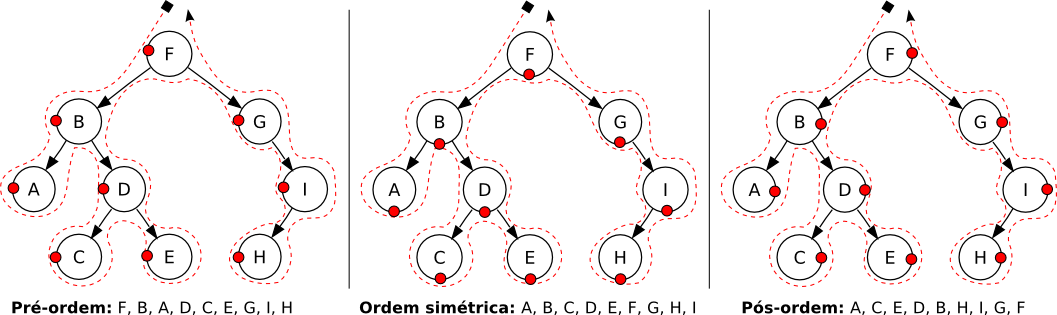
\includegraphics[width=350pt]{imagens/percurso.png}
  \label{fig_percurso}
\end{figure}
\end{frame}

\begin{frame}{Árvore Binária}{Percurso em Árvore - Exercício}
Considere a arvore a seguir:
\begin{figure}[!h]
  \centering
  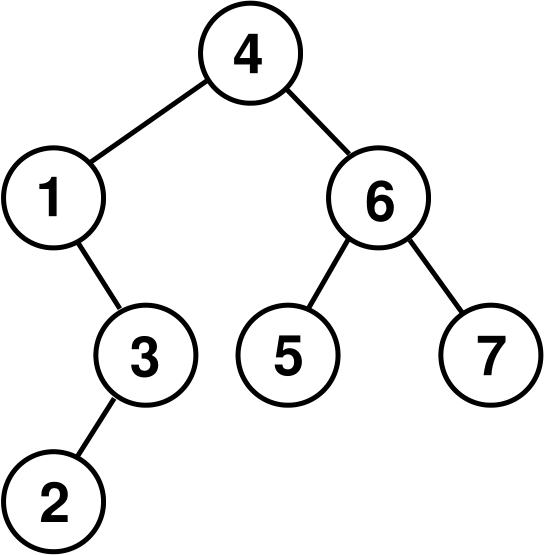
\includegraphics[width=120pt]{imagens/exercicio1.png}
  \label{fig_exercicio1}
\end{figure}
Qual a ordem de visitação dos nodos utilizando o percurso:
\begin{itemize}
 \item Pré-ordem.
 \item Em-ordem.
 \item Pós-ordem.
\end{itemize}
\end{frame}

\begin{frame}{Árvore Binária}{Percurso em Árvore - Exercício}
Considere a arvore a seguir:
\begin{figure}[!h]
  \centering
  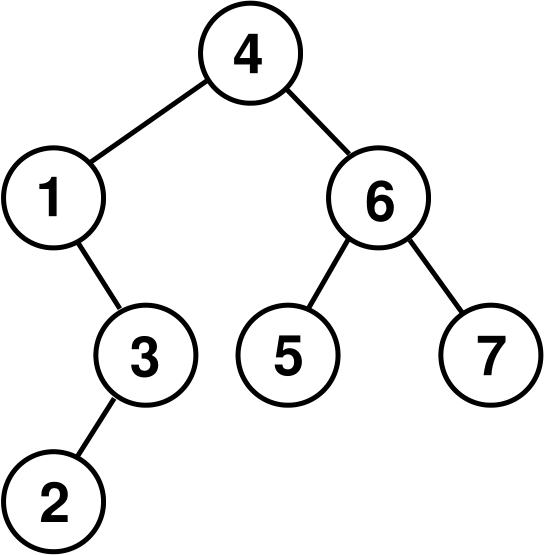
\includegraphics[width=120pt]{imagens/exercicio1.png}
\end{figure}
Qual a ordem de visitação dos nodos utilizando o percurso:
\begin{itemize}
 \item Pré-ordem. {\bf 4, 1, 3, 2, 6, 5, 7}
 \item Em-ordem. {\bf 1, 2, 3, 4, 5, 6, 7}
 \item Pós-ordem. {\bf 2, 3, 1, 5, 7, 6, 4}
\end{itemize}
\end{frame}

% -----------------------------------


%\begin{frame}{Dúvidas}
%\Huge{\centerline{Dúvidas?}}
%
%\begin{figure}[!h]
%  \centering
%  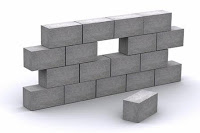
\includegraphics[width=100pt]{imagens/duvidas.jpg}
%  \label{fig_fim}
%\end{figure}
%\end{frame}

\begin{frame}{Referências}{Bibliografia Básica}

\begin{itemize}
\item Bibliografia Básica
\bibliographystyle{abnt-alf}
\bibliography{referencias}
\item Material Complementar
\begin{itemize}
\item \href{https://programacaodescomplicada.wordpress.com/complementar/}{Link código-fonte e listas de exercícios- Material disponível on-line}
\end{itemize}
\item Vídeo-aulas
\begin{itemize}
\item \href{https://www.youtube.com/watch?v=iLvpaqAoVD8&index=67&list=PL8iN9FQ7_jt6H5m4Gm0H89sybzR9yaaka&t=106s}{Curso de programação e estrutura de dados em linguagem C}
\item \href{https://www.youtube.com/watch?v=eiMMtyRBYCE&list=PLxI8Can9yAHf8k8LrUePyj0y3lLpigGcl&index=15}{Estrutura de dados - Univesp}
\end{itemize}
%\item Animação
%\begin{itemize}
%\item \href{https://www.cs.usfca.edu/~galles/visualization/BST.html}{Link Árvore Binária de Busca}
%\item \href{http://btv.melezinek.cz/binary-search-tree.html}{Link Árvore Binária de Busca - Versão que utiliza sucessor como nodo subtituto na remoção.}
%\end{itemize}
\end{itemize}
\end{frame}


%------------------------------------------------
\begin{frame}
\titlepage % Print the title page as the first slide

\begin{figure}[!h]
  \centering
   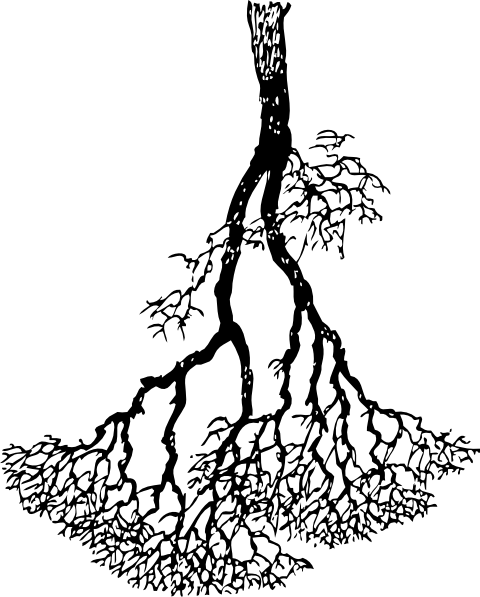
\includegraphics[width=80pt]{imagens/introducao.png}
  \label{fig_introducao}
\end{figure}
\end{frame}
%----------------------------------------------------------------------------------------


\end{document} 
